% example tikz figure

\documentclass{article}

\usepackage{tikz}
\usetikzlibrary{arrows,shapes,positioning,shadows,trees}


\begin{document}

\begin{tikzpicture}
    % x axis, length 10
    \draw[-] (-3,0) -- (5,0);
    % origin
    \node[fill,circle,inner sep=1pt,label=below:$O$] at (0,0) {};
    % R at (4,0) and (-2,0), circle with arrow
    \draw[->] (4,0.2) arc (0:185:3);
    % another half
    \draw[->] (-2,0) arc (180:355:3);
    % small circle at (0,0), radius 1
    % \draw (0,0) circle (1);
    \draw[<-] (1,0.2) arc (10:180:1);
    \draw[<-] (-1,0) arc (180:350:1);

    % -1
    \node[fill,circle,inner sep=1pt,label=below:$-1$] at (-1.5,0) {};
    % R
    \node[fill,circle,inner sep=1pt,label=above right:$R$] at (4,0) {};

    % connect two circles with [1,4] x {\pm \epsilon}
    \draw[->] (1,0.2) -- (4,0.2);
    \draw[<-] (1,-0.2) -- (4,-0.2);
\end{tikzpicture}

\begin{tikzpicture}
    % origin
    \node[fill,circle,inner sep=1pt,label=below:$O$] at (0,0) {};

    % radius 1 circle, top half
    \draw[<-] (1,0) arc (0:180:1);
    % (1,0) -> (4,0) and reverse
    \draw[->] (1,0) -- (4,0);
    \draw[<-] (-1,0) -- (-4,0);

    % radius 4 circle, top half
    \draw[<-] (4,0) arc (0:180:4);

    % \pm \rho at (\pm 1,0)
    \node[fill,circle,inner sep=1pt,label=below:$-\rho$] at (-1,0) {};
    \node[fill,circle,inner sep=1pt,label=below:$\rho$] at (1,0) {};

    % \pm R at (\pm 4,0)
    \node[fill,circle,inner sep=1pt,label=below:$-R$] at (-4,0) {};
    \node[fill,circle,inner sep=1pt,label=below:$R$] at (4,0) {};

    % \gamma_R
    \node[label=above right:$\gamma_R$] at (4 * 0.6,4 * 0.8) {};

    % \gamma_\rho
    \node[label=above right:$\gamma_\rho$] at (1 * 0.6,1 * 0.8) {};

    % label i at (0,3)
    \node[fill,circle,inner sep=1pt,label=right:$i$] at (0,2.5) {};
\end{tikzpicture}


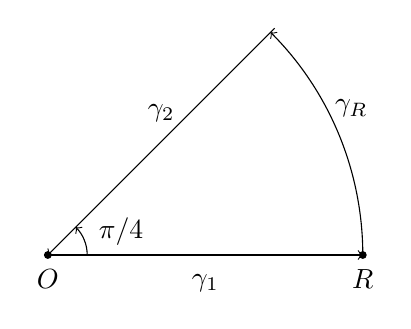
\begin{tikzpicture}
    % 0 to R \gamma_1
    \draw[->] (0,0) -- (4,0);
    \node[fill,circle,inner sep=1pt,label=below:$O$] at (0,0) {};
    \node[fill,circle,inner sep=1pt,label=below:$R$] at (4,0) {};
    \node[label=below:$\gamma_1$] at (2,0) {};

    % R to R' which rotates pi/4 from origin, \gamma_R
    \draw[->] (4,0) arc (0:45:4);
    \node[label=above right:$\gamma_R$] at (3.4, 1.5) {};

    % R' to origin \gamma_2
    \draw[->] (4 * 0.72,4*0.72) -- (0,0);
    \node[label=above:$\gamma_2$] at (2 * 0.72, 2 * 0.72) {};

    % label angle with \pi / 4, use a small arc to denote
    \draw[->] (0.5,0) arc (0:45:0.5);
    \node[label=right:$\pi/4$] at (0.5 * 0.8, 0.5 * 0.6) {};
\end{tikzpicture}

\begin{tikzpicture}
    % x-axis with length 8
    \draw[-] (-4,0) -- (4,0);
    % origin, -R&R at (-3,0)&(3,0)
    \node[fill,circle,inner sep=1pt,label=below:$O$] at (0,0) {};
    \node[fill,circle,inner sep=1pt,label=below:$-R$] at (-3,0) {};
    \node[fill,circle,inner sep=1pt,label=below:$R$] at (3,0) {};

    % y-axis with length 3, only +y
    \draw[->] (0,0) -- (0,2.5);

    % \gamma_1 from R to (3,2)
    \draw[->] (3,0) -- (3,1);
    \draw[-] (3,1) -- (3,2);
    \node[label=above right:$\gamma_1$] at (3,1) {};

    % \gamma_2 from (3,2) to (-3,2)
    \draw[->] (3,2) -- (2,2);
    \draw[-] (2,2) -- (-3,2);
    \node[label=above right:$\gamma_2$] at (2,2) {};

    % \gamma_3 from (-3,2) to (-3,0)
    \draw[->] (-3,2) -- (-3,1);
    \draw[-] (-3,1) -- (-3,0);
    \node[label=above left:$\gamma_3$] at (-3,1) {};

    \node[label=above right:$R+\frac{b}{2a}i$] at (3,2) {};
\end{tikzpicture}
\end{document}